\documentclass{article}
\input{../../../LaTex/preamble/preamble_article.tex}

\begin{comment}
    重复语句
   

\end{comment}


\title{高物选修3-2 \quad 交流电}
\author{马祥芸}

\begin{document}
    \maketitle
    \tableofcontents
    \newpage

    \section{交流电}  

    \subsection{交流电介绍}

    \begin{enumerate}
        \item 电流分类
        \begin{enumerate}[label=(\arabic*)]
            \item 恒定电流: \quad \textbf{$I$大小恒定,且方向不变}
            \item 直流电: \quad \textbf{仅方向不变}
            \item 交流电: \quad \textbf{方向改变(唯一判据)}
        \end{enumerate}

        \item 认识交变电流
        \begin{enumerate}[label=(\arabic*)]
            \item 电流大小的改变
            \begin{figure}[h] %[h]表示当前图片位置在代码位置
                \centering
                
                \begin{subfigure}{0.4\textwidth}
                    \centering
                    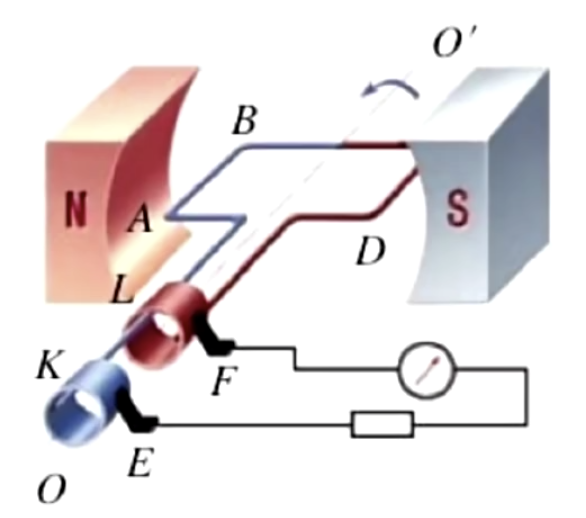
\includegraphics[width=\textwidth,keepaspectratio]{pictures/1.1-1.png}
                    \caption{} % 添加子图 A 的标题
                \end{subfigure}
                \hfill % 添加水平间距              
                %空行会被解释为段落结束的标志,因此如果在 subfigure 环境之间添加了空行,就会被视为新的段落,从而导致两个 subfigure 不再处于同一行上。
                \begin{subfigure}{0.4\textwidth}
                    \centering
                    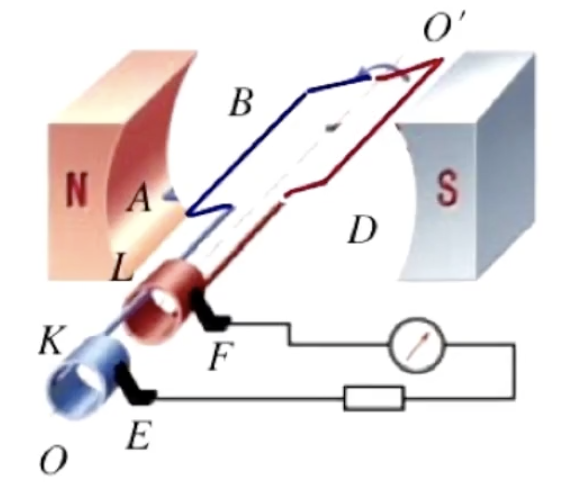
\includegraphics[width=\textwidth,keepaspectratio]{pictures/1.1-2.png}
                    \caption{} % 添加子图 B 的标题
                \end{subfigure}
            \end{figure}

            原因: \quad 切割磁感线的分速度随着旋转发生\textbf{大小的改变}

            \vspace{5em}

            \item 电流方向的改变
            
            \begin{figure}[h] %[h]表示当前图片位置在代码位置
                \centering
                
                \begin{subfigure}{0.4\textwidth}
                    \centering
                    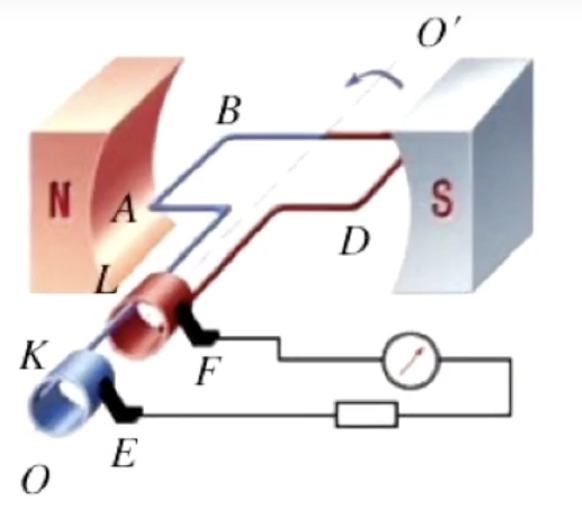
\includegraphics[width=\textwidth,keepaspectratio]{pictures/1.1-3.png}
                    \caption{} 
                \end{subfigure}
                \hfill % 添加水平间距              
                %空行会被解释为段落结束的标志,因此如果在 subfigure 环境之间添加了空行,就会被视为新的段落,从而导致两个 subfigure 不再处于同一行上。
                \begin{subfigure}{0.4\textwidth}
                    \centering
                    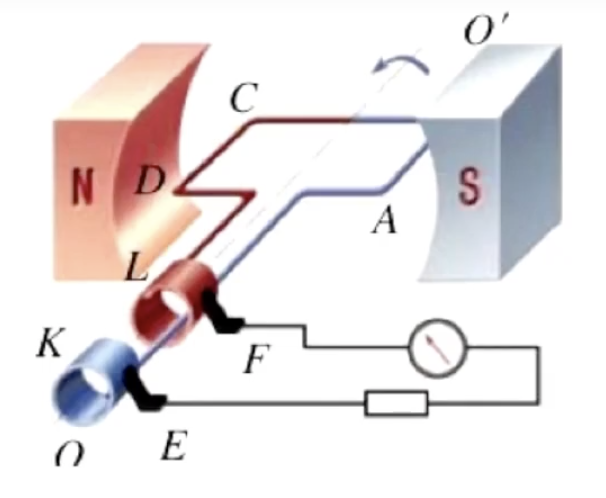
\includegraphics[width=\textwidth,keepaspectratio]{pictures/1.1-4.png}
                    \caption{} 
                \end{subfigure}
            \end{figure}
            原因: \quad 切割磁感线的分速度随着旋转发生\textbf{方向的改变}
        \end{enumerate}

    \end{enumerate}


\begin{comment}
    \subsection{中性面及其特点}

    \section{四值}
    
    \subsection{瞬时值和最大值}

    \subsection{有效值和平均值}

    \subsection{有效果值的解题计算}

    \section{小结}

    \subsection{交流电的例题讲解}

    \section{自感和电容对交流电的影响}

\end{comment}


\end{document}